\section{Examples}

%%------------------------------------------------------------ SUBSECTION ---------------------
\subsection{Example: One-Mass-Oscillator With Recursive Structure and Impact}

\hspace*{0.2\hsize}
  %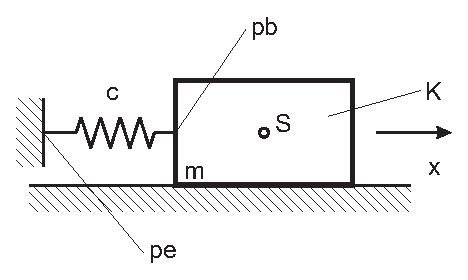
\includegraphics[width=0.45\hsize]{mbsim_one_mass_oscillator.eps}

%%------------------------------------------------------------ SUBSUBSECTION ---------------------
\subsubsection{Physics - system}

\paragraph{Header}

\lstinputlisting{C++/system.h}

\begin{tabular}{r|p{0.85\hsize}}
  1,2,13 & avoids including Header more than once\\
  4,5  & \emph{includes}\\
  7 & class definition for one mass oscillator, which is derived by \texttt{DynamicSystemSolver} without additional functionality\\
  9 & constructor
\end{tabular}

%------------------------------------------------------------
\paragraph{Source}

\lstinputlisting{C++/system.cc}

%%------------------------------------------------------------ SUBSUBSECTION ---------------------
\subsubsection{Time integration -- main}

\lstinputlisting{C++/main.cc}

%%------------------------------------------------------------ SUBSUBSECTION ---------------------
\subsubsection{Makefile} \enlargethispage{5mm}
The building process of a program is controlled by a Makefile:
\lstinputlisting{C++/Makefile}

%%--------------------------------------------------------------- SUBSECTION --
\subsection{2D-Slider Crank Mechanism}
Use the following plan.
\begin{enumerate}
\item rigid bodies with
\begin{itemize}
\item \emph{RigidBody} for crank, pistin and block
\item mass/ length/ width/ inertia tensor
\item Jacobian matrices (translation / rotation)
\item reference frames
\item \OpenMBV{}-bodies (probably one needs an additional translation as \OpenMBV{}-bodies sometimes use another reference)
\end{itemize}

\item elastic connecting rod with
\begin{itemize}
\item \emph{FlexibleBody1s21RCM}
\item length/ width / height (cross-sectional area) / Young's modulus (10e8)/ area moment of inertia / density/ damping
\item number of finite elements
\item reference frames
\item initial generalised coordinates
\end{itemize}

\item frames/ contours in body coordinate system
\item link definition
\item external loads
\item add to dynamic system solver
\item integrator / time step size
\end{enumerate}

%%--------------------------------------------------------------- SUBSECTION --
\subsection{3D-Slider Crank Mechanism}
Use the following plan.
\begin{enumerate}
\item rigid bodies with
\begin{itemize}
\item \emph{RigidBody} for crank, connecting rod, piston and block
\item mass/ length/ width / inertia tensor
\item Jacobian matrices (translation / rotation)
\item reference frames
\item \OpenMBV{}-bodies
\end{itemize}

\item frames / contours in body coordinate system
\item link definition
\item external loads
\item add to dynamic system solver
\item integrator / time step size
\end{enumerate}


